\documentclass[11pt]{article}
\usepackage[T1]{fontenc}
\usepackage{lmodern}
\usepackage[a4paper,margin=28mm]{geometry}
\usepackage{amsmath,amssymb,amsthm,mathtools,microtype,booktabs,array}
\usepackage{tikz}
\usetikzlibrary{arrows.meta}
\usepackage{xurl}
\usepackage[hidelinks,pdfusetitle]{hyperref}
\ifdefined\pdfglyphtounicode
  \pdfgentounicode=1
  \pdfglyphtounicode{tfm:lmsy10/mapsto}{007C}
  \pdfglyphtounicode{tfm:lmex10/parenleftbig}{0028}
  \pdfglyphtounicode{tfm:lmex10/parenrightbig}{0029}
  \pdfglyphtounicode{tfm:lmex10/floorleftbigg}{230A}
  \pdfglyphtounicode{tfm:lmex10/floorrightbigg}{230B}
  \pdfglyphtounicode{tfm:lmex10/parenleftBigg}{0028}
  \pdfglyphtounicode{tfm:lmex10/parenrightBigg}{0029}
  \pdfglyphtounicode{tfm:lmex10/summationtext}{2211}
  \pdfglyphtounicode{tfm:lmex10/integraltext}{222B}
  \pdfglyphtounicode{tfm:lmex10/summationdisplay}{2211}
  \pdfglyphtounicode{tfm:lmex10/integraldisplay}{222B}
  \pdfglyphtounicode{tfm:lmex10/uniondisplay}{22C3}
  \pdfglyphtounicode{tfm:lmex10/braceleftBig}{007B}
  \pdfglyphtounicode{tfm:lmex10/bracerightBig}{007D}
  \pdfglyphtounicode{tfm:lmex10/radicalbig}{221A}
  \pdfglyphtounicode{tfm:lmex10/radicalBig}{221A}
\fi
\newtheorem{theorem}{Theorem}[section]
\newtheorem{lemma}[theorem]{Lemma}
\newtheorem{proposition}[theorem]{Proposition}
\newtheorem{corollary}[theorem]{Corollary}
\theoremstyle{remark}
\newtheorem{remark}[theorem]{Remark}
\newcommand{\R}{\mathbb R}
\newcommand{\Z}{\mathbb Z}
\newcommand{\Cyl}{\mathcal C}
\newcommand{\area}{\operatorname{area}}
\newcommand{\dist}{\operatorname{dist}}
\newcommand{\tr}{\operatorname{tr}}
\numberwithin{equation}{section}
\setlength{\emergencystretch}{2em}
\title{Finite cylinder approximation of ruled sets}
\author{OpenAI}
\date{September 27, 2026}
\begin{document}
\maketitle
\begin{abstract}
We approximate compact ruled families of segments by finitely many
cylinders with square intercept tiles and perpendicular-base area at
most their integral projection cost plus any positive error. The
velocity field is $C^1$, and its differential has opposite real
eigenvalues whose magnitudes are strictly below the inverse segment
half-length; both eigenvalues may vanish. The result includes
square-zero differentials with unrestricted shear and fields that
pass between the two regimes. It holds for arbitrary compact label
sets.
\end{abstract}
\section{The finite approximation problem}\label{b:introduction}
A cylinder in $\R^3$ is a set $B+\R u$, where $u$ is a Euclidean unit
vector and $B\subset u^\perp$ is measurable with finite area. Its cost is
$|B|$; the cost of a finite family is the sum of these areas, counted with
multiplicity. A continuously varying family of segments suggests a way to
choose economical directions. Turning it into finitely many cylinders is
a separate problem: simply freezing a direction on each small label patch
can open gaps or create an area loss that does not vanish with the mesh.

The motivation comes from cylinder coverings of convex bodies. If
$K\subset\R^3$ is a compact convex set with nonempty interior, write
$A_{\min}(K)=\min_{|u|=1}|\pi_{u^\perp}K|$ for its smallest orthogonal
projection area. Bezdek records a question attributed to Bang asking
whether every finite cylinder cover costs at least $A_{\min}(K)/2$, together
with a two-cylinder equality example for the regular tetrahedron
\cite[Problem~3.1]{Bezdek2009}. Bezdek and Litvak prove the universal
lower bound $A_{\min}(K)/3$ in dimension three as a consequence of their
stronger directionwise normalized inequality
\cite[Theorem~3.1]{BL2009}. A useful way to search for inexpensive covers is
to perturb the lines in a simple configuration, compare the added label
area with the saving in perpendicular projection, and only then make the
family finite. This paper supplies that last step with its exact
hypotheses and area factor.

\subsection{Segments, tiles, and their Euclidean cost}
We use an axial coordinate $s\in\R$ and transverse coordinates
$p=(p_1,p_2)\in\R^2$. For a compact set $D\subset\R^2$, a continuous
field $V$ defined near $D$, and $L>0$, set
\begin{equation}\label{b:ruled-set}
 E(D,V,L)=\{(s,p+sV(p)):p\in D,\ |s|\le L\}.
\end{equation}
The label $p$ is the intercept at $s=0$ and $(1,V(p))$ is the
segment direction. A measurable tile $T\subset\R^2$ and a constant
velocity $g\in\R^2$ determine
\[
 \Cyl(T,g)=\{(s,\xi):s\in\R,\ \xi\in T+sg\}.
\]
At each height its section is a translate of $T$, rather than a deformed
copy. These are the cylinders used in our finite covers.

For a fixed $h>0$, allow the physical coordinate map
\[
 F_h(s,\xi)=(s,\xi_1,h\xi_2),\qquad
 J_h(g)=(1+g_1^2+h^2g_2^2)^{-1/2}.
\]
When $h=1$ the coordinates are orthonormal.
Throughout, a velocity's components in $J_h$ refer to these original
coordinates, even when the tile is rotated.

\begin{proposition}[Perpendicular base area]\label{b:projection}
Let $h>0$, let $T\subset\R^2$ be bounded and measurable, and let
$g\in\R^2$. The image $F_h(\Cyl(T,g))$ is a cylinder whose perpendicular
base has area $h|T|J_h(g)$. A compact nondegenerate parallelogram tile
has a compact nondegenerate parallelogram base. An open tile gives an
open base. The formula is unchanged after a Euclidean isometry.
\end{proposition}
\begin{proof}
The intercept tile $F_h(\{0\}\times T)$ has physical area $h|T|$ and
lies in the plane with unit normal $(1,0,0)$. Its cylinder direction is
$v=(1,g_1,hg_2)$. Orthogonal projection onto $v^\perp$ has constant area
Jacobian $|(1,0,0)\cdot v/|v||=J_h(g)$ on the intercept plane: this follows
by projecting an orthonormal pair and taking the area of its parallelogram.
A point and its projection differ by a multiple of $v$, so the projected
tile sweeps precisely the same cylinder. The projection is an invertible
linear map between the two planes because the first component of $v$ is
nonzero. It preserves compactness, openness, and nondegeneracy as asserted.
Isometries preserve perpendicular area and the cylinder property.
\end{proof}

Thus the prospective cost of the physical family $F_h(E(D,V,L))$ is
$h\int_D J_h(V(p))\,dp$. The following theorem realizes this upper
bound to arbitrary accuracy with square intercept tiles.

\begin{theorem}[Finite approximation by square tiles]\label{b:approximation}
Let $D\subset\R^2$ be compact, let $V$ be $C^1$ on an open
neighborhood of $D$, and let $L,h>0$. Suppose that
\begin{equation}\label{b:main-condition}
 \tr DV(p)=0,\qquad -L^{-2}<\det DV(p)\le0
 \quad(p\in D).
\end{equation}
For every $\varepsilon>0$, there are finitely many compact
nondegenerate square tiles $T_i\subset\R^2$, with possibly different
orientations, and velocities $g_i\in\R^2$ such that
\begin{equation}\label{b:main-cover}
 E(D,V,L)\subset\bigcup_i\Cyl(T_i,g_i),\qquad
 \sum_i |T_i|J_h(g_i)
 \le\int_D J_h(V(p))\,dp+\varepsilon.
\end{equation}
Under $F_h$, the perpendicular bases are compact nondegenerate
parallelograms and have total area $h\sum_i|T_i|J_h(g_i)$.
No condition on the area of $\partial D$ or smallness of $\|DV\|$
is required.
\end{theorem}

To obtain a prescribed error in physical base area, use that error
divided by $h$ as $\varepsilon$ in \eqref{b:main-cover}. The construction
includes compact label sets of area zero or with positive-area boundary.
The velocities $g_i$ are chosen from local affine approximations to $V$;
they need not equal the original field at the tile centers.

The eigenvalues in \eqref{b:main-condition} are
$\lambda_p,-\lambda_p$, where $\lambda_p=\sqrt{-\det DV(p)}$ and
$0\le L\lambda_p<1$. Thus opposite nonzero real eigenvalues are
allowed up to the strict length bound. When $\lambda_p=0$,
Cayley--Hamilton gives $(DV(p))^2=0$. In particular, a field with
square-zero differential everywhere on $D$ satisfies the theorem for
every fixed $L>0$, with no bound on its shear coefficient. The two types
may occur in the same field: for
\[
 V(p_1,p_2)=(p_2,p_1^3/3),\qquad
 DV(p)=\begin{pmatrix}0&1\\p_1^2&0\end{pmatrix},
\]
the theorem applies on any compact subset of $|p_1|<L^{-1}$.
The differential is square-zero on $p_1=0$ and hyperbolic elsewhere.

\subsection{Why fixed squares suffice}
For an affine field with derivative $A$, label differences at height
$s$ are transformed by $I+sA$. A trace-zero planar matrix has an
orthonormal basis in which its diagonal vanishes. In those coordinates,
write $A=\left(\begin{smallmatrix}0&b\\c&0\end{smallmatrix}\right)$.
The unit-grid centers then move to
\[
 (i+sbj,\,sci+j),\qquad(i,j)\in\Z^2.
\]
The squares themselves keep their sides and their area. They still
cover the entire plane whenever $0\le s^2bc<1$, even if an individual
coefficient $sb$ or $sc$ is large. A direct rounded fixed-point argument
proves this covering in Section~\ref{b:linear-coverings}. When one
coefficient is zero, the motion simply slides the rows or columns.

The bounded-parameter square covering is related to Stein's
notched-square construction in Kolountzakis's formulation
\cite[Theorem~7]{Kolountzakis1998}. The full positive-product range also
follows from the signed-function identity in the same paper
\cite[Section~2.3, equations~(17)--(20)]{Kolountzakis1998}.
We give an elementary proof, including the zero-product cases and all
square boundaries. Its integer iteration is a finite-chain instance of
Tarski's monotone fixed-point principle~\cite[Theorem~1]{Tarski1955}.
These comparisons concern the affine covering; the finite nonlinear
construction and its area estimate are proved here.

Section~\ref{b:finite-proof} passes to a $C^1$ field. On each coarse
square meeting $D$, we freeze an affine approximation and use a much
finer square grid in its orthonormal coordinates. The infinite affine
cover contains every actual nonlinear target. The inverse of $I+sA$
then shows that only centers in a thin collar of the coarse square are
needed, uniformly over the allowed heights. The fine-grid spacing and
the Taylor error both make that collar thinner than the coarse side
length by a factor tending to zero. Its extra tile area is therefore
negligible. Summing the sampled weights over the coarse squares gives
the integral over a shrinking outer neighborhood of $D$, which converges
to the integral over $D$ without a boundary-regularity assumption.

Section~\ref{b:product-section} develops a different construction with
open intercept cells bounded by hyperbolas. Their long arms absorb
expansion in one eigendirection and contraction in the other at small
relative area cost. This method packs the interior and requires a label
set with area-zero boundary; logarithmic dilation gives a finite-stopping
variant of the same construction. These alternatives are not needed for
Theorem~\ref{b:approximation}. Section~\ref{b:comparison} discusses
physical rescaling, the role of the spectral bound, and the use of a
finite approximation within a later parameter limit.

\section{Square coverings for affine motion}\label{b:linear-coverings}

We first cover the whole transverse plane for a frozen affine velocity
field. The squares keep their side lengths and orientations; only their
centers move. An inverse estimate will then locate the centers needed
near a compact set of labels. Neither step requires a smallness bound on the
individual shear coefficients.

\begin{lemma}[A deformed square grid]\label{b:lattice}
Let $\alpha,\beta\in\R$ satisfy $0\le\alpha\beta<1$.
The closed unit squares with centers
\[
 (i+\alpha j,\,\beta i+j),\qquad (i,j)\in\Z^2,
\]
cover $\R^2$.
\end{lemma}
\begin{proof}
Write $R(t)=\lfloor t+1/2\rfloor$. For a target $u=(u_1,u_2)$,
it suffices to find integers satisfying
\[
 i=R(u_1-\alpha j),\qquad j=R(u_2-\beta i).
\]
Consider $F(i)=R(u_1-\alpha R(u_2-\beta i))$. If
$\alpha\beta>0$, the two multiplications either both preserve or
both reverse order, so $F$ is nondecreasing. If either coefficient
is zero, $F$ is constant and hence still nondecreasing. Moreover,
\[
 F(i)=\alpha\beta i+O(1)\qquad(|i|\to\infty).
\]
Since $\alpha\beta<1$, there are integers $i_-<i_+$ with
$F(i_-)\ge i_-$ and $F(i_+)\le i_+$. Monotonicity makes the
finite integer interval between them invariant. Iteration from $i_-$
is nondecreasing and bounded, so it reaches a fixed point. Setting
$j=R(u_2-\beta i)$ gives the required pair. Each coordinate error
is at most $1/2$, including equality at the square boundaries.
\end{proof}

This iteration is a finite-chain instance of Tarski's monotone
fixed-point principle \cite[Theorem~1]{Tarski1955}. The positive-product
covering also follows from the signed tiling identity of Kolountzakis
\cite[Section~2.3, equations~(17)--(20)]{Kolountzakis1998}.
After taking its parameters to be $|\alpha|,|\beta|$ and reflecting
one coordinate when necessary, that identity gives the lattice sum of
a unit-square indicator minus a rectangle indicator as $1$ almost
everywhere. The rectangle contribution is nonnegative, so the squares
cover almost everywhere. Their closed, locally finite union then
covers every point. When both parameters have absolute value below
one, Stein's notched-square construction already supplies this
covering \cite[Theorem~7 and equations~(13)--(14)]{Kolountzakis1998}.
The direct proof above includes the zero-product cases as well.

\begin{lemma}[An orthogonal zero-diagonal basis]\label{b:zero-diagonal}
Let $A$ be a real $2\times2$ matrix with $\tr A=0$.
There is an orthonormal basis in which
\[
 A=\begin{pmatrix}0&b\\c&0\end{pmatrix},\qquad bc=-\det A.
\]
\end{lemma}
\begin{proof}
For a unit vector $e$, let $e^\perp$ be its counterclockwise
quarter-turn and put $q(e)=e^{\mathsf T}Ae$. The trace identity
gives $q(e)+q(e^\perp)=0$. Continuity on the quarter-circle
between these vectors supplies a unit vector with $q(e)=0$.
Then $q(e^\perp)=0$ also. The determinant gives the formula for
the product of the off-diagonal entries.
\end{proof}

\begin{lemma}[Affine square covering and center control]\label{b:affine-cover}
Let $L>0$ and let $A$ be a real $2\times2$ matrix satisfying
\[
 \tr A=0,\qquad -L^{-2}<\det A\le0.
\]
Fix $p_0,v_0\in\R^2$ and write $W(p)=v_0+A(p-p_0)$.
There is an orthonormal basis $e_1,e_2$ such that, for every
$\tau>0$, the lattice
\[
 \Lambda=p_0+\tau\Z e_1+\tau\Z e_2
\]
and its closed squares
\[
 T_l=l+[-\tau/2,\tau/2]e_1+[-\tau/2,\tau/2]e_2
 \qquad(l\in\Lambda)
\]
satisfy
\[
 \R^2=\bigcup_{l\in\Lambda}\bigl(T_l+sW(l)\bigr)
 \qquad(|s|\le L).
\]
If $x$ belongs to the translated tile indexed by $l$, then
$|x-l-sW(l)|\le\tau$. Furthermore,
\begin{equation}\label{b:affine-inverse}
 \|(I+sA)^{-1}\|
 \le \frac{1+L\|A\|}{1+L^2\det A}
 \qquad(|s|\le L),
\end{equation}
where the norm is the Euclidean operator norm.
\end{lemma}
\begin{proof}
Choose the basis from Lemma~\ref{b:zero-diagonal}. After subtracting
$p_0+sv_0$ and using this basis in units of $\tau$, the centers are
\[
 (i+sbj,\,sci+j).
\]
Their two parameters have product $s^2bc=-s^2\det A\in[0,1)$,
so Lemma~\ref{b:lattice} applies. The distance from a point of a
square to its center is at most $\tau/\sqrt2$, giving the stated
bound. Cayley--Hamilton and $\tr A=0$ give
\[
 A^2=-(\det A)I,\qquad
 (I+sA)^{-1}=\frac{I-sA}{1+s^2\det A}.
\]
The denominator is at least $1+L^2\det A>0$, which proves
\eqref{b:affine-inverse}.
\end{proof}

Figure~\ref{b:figure-lattice} shows the case of equal positive
off-diagonal parameters. In the affine covering, the tiles keep their
area even though the center map has determinant
$1+s^2\det A\le1$.

\begin{figure}[tb]
\centering
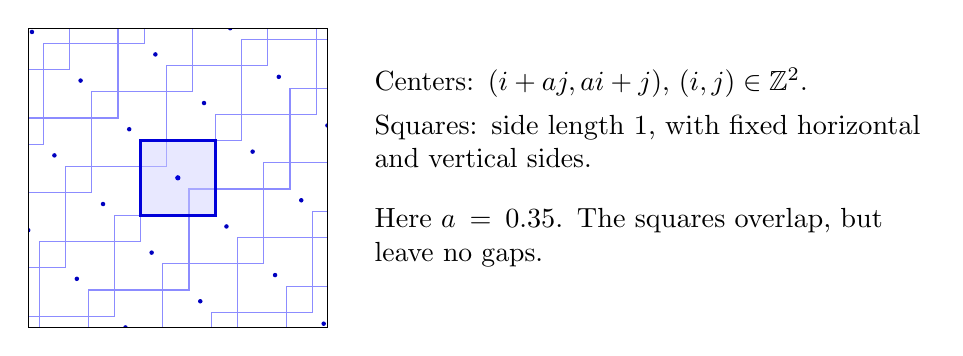
\begin{tikzpicture}[scale=0.95]
 \begin{scope}
  \clip (-2,-2) rectangle (2,2);
  \foreach \i in {-4,...,4} {\foreach \j in {-4,...,4} {
   \pgfmathsetmacro{\cx}{\i+.35*\j}
   \pgfmathsetmacro{\cy}{\j+.35*\i}
   \draw[blue!45,line width=.4pt]
     ({\cx-.5},{\cy-.5}) rectangle ({\cx+.5},{\cy+.5});
   \fill[blue!75!black] (\cx,\cy) circle (.03);
  }}
  \fill[blue!20,opacity=.45] (-.5,-.5) rectangle (.5,.5);
  \draw[blue!85!black,line width=1.1pt] (-.5,-.5) rectangle (.5,.5);
  \fill[blue!85!black] (0,0) circle (.035);
 \end{scope}
 \draw (-2,-2) rectangle (2,2);
 \node[align=left,anchor=west,text width=7cm] at (2.5,.8)
   {Centers: $(i+aj,ai+j)$, $(i,j)\in\Z^2$.\\[4pt]
    Squares: side length $1$, with fixed horizontal and vertical sides.};
 \node[align=left,anchor=west,text width=7cm] at (2.5,-.8)
   {Here $a=0.35$. The squares overlap, but leave no gaps.};
\end{tikzpicture}
\caption{A bounded window in the lattice covering of
Lemma~\ref{b:lattice}, with the square at the origin highlighted.
The squares keep their original shape and orientation as their centers move.
The affine construction uses an orthonormal basis for each frozen
differential. Its finite approximation retains fine-grid centers only
near the corresponding coarse label square.}
\label{b:figure-lattice}
\end{figure}


The square-zero case has a particularly simple interpretation. If
$A\ne0$ and $A^2=0$, then $\operatorname{im}A=\ker A$ is a line.
Choose $e_1$ along that line. In an orthonormal basis the map is
$(x,y)\mapsto(dy,0)$ for some $d\in\R$. After removing the common
translation, row $j$ of the square lattice moves horizontally by
$sd\tau j$. Its vertical interval stays fixed, and the horizontal
intervals in each row still cover the line. Thus the squares cover
for every $s\in\R$ and every $d$, as illustrated in
Figure~\ref{b:figure-rows}. For $A=0$ this is the ordinary square
grid. This explains directly why no bound on the shear is needed
in the square-zero case.

\begin{figure}[ht]
\centering
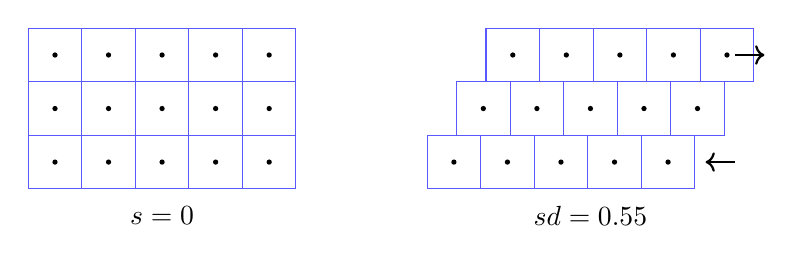
\begin{tikzpicture}[scale=.68]
 \begin{scope}
  \foreach \j in {-1,0,1} {
   \foreach \i in {-2,-1,0,1,2} {
    \draw[blue!65] (\i-.5,\j-.5) rectangle (\i+.5,\j+.5);
    \fill (\i,\j) circle (1.4pt);
   }
  }
  \node at (0,-2.0) {$s=0$};
 \end{scope}
 \begin{scope}[xshift=8cm]
  \foreach \j in {-1,0,1} {
   \foreach \i in {-2,-1,0,1,2} {
    \draw[blue!65] (\i+.55*\j-.5,\j-.5) rectangle (\i+.55*\j+.5,\j+.5);
    \fill (\i+.55*\j,\j) circle (1.4pt);
   }
  }
  \draw[->,thick] (2.7,1) -- (3.25,1);
  \draw[->,thick] (2.7,-1) -- (2.15,-1);
  \node at (0,-2.0) {$sd=0.55$};
 \end{scope}
\end{tikzpicture}
\caption{Sliding rows with $\tau=1$, after removing the common
translation. The tiles remain squares while row $j$ moves horizontally
by $sdj$. Each drawing shows a finite portion of a grid extending
infinitely in both directions. No gaps arise between the closed rows.}
\label{b:figure-rows}
\end{figure}


\section{From affine coverings to a finite family}\label{b:finite-proof}

We prove Theorem~\ref{b:approximation}. On each coarse label square,
freeze the field to its affine approximation and use a much finer
square lattice. The affine covering captures the actual nonlinear
target point; its inverse estimate shows that only a thin collar of
extra centers is needed. We then estimate the cost one coarse square
at a time. Overlaps between different coarse squares are counted
with multiplicity.

\begin{proof}[Proof of Theorem~\ref{b:approximation}]
If $D=\varnothing$, take the empty collection. Otherwise fix $L,h>0$
as in the theorem. Compactness and the strict determinant bound give
\[
 \sigma=\min_{p\in D}\bigl(1+L^2\det DV(p)\bigr)>0.
\]
Choose $a>0$ so that the compact neighborhood
$D_a=\{p:\dist(p,D)\le a\}$ is contained in the domain of $V$.
Let $M$ bound $\|DV\|$ on $D_a$, and let $\omega(r)$ be the
supremum of $\|DV(x)-DV(y)\|$ over $x,y\in D_a$ with
$|x-y|\le r$. Then $\omega(r)\to0$ as $r\downarrow0$.
Set
\[
 C=\frac{1+LM}{\sigma}.
\]
By \eqref{b:affine-inverse}, this bounds the inverse of every frozen
map $I+sDV(p)$ for $p\in D$ and $|s|\le L$, including labels
where the derivative is square-zero or zero.

\paragraph{The coarse squares and their affine fields.}
Take all closed squares $S$ of side $\delta$ in a fixed square
grid that meet $D$, and choose $b_S\in S\cap D$. There are
finitely many such squares. For all sufficiently small $\delta$
they lie in $D_a$. Put
\[
 A_S=DV(b_S),\qquad V_S(p)=V(b_S)+A_S(p-b_S).
\]
The spectral hypotheses are used at $b_S\in D$ only; no such
conditions are needed on the surrounding neighborhood. Integrating
$DV$ along the segment from $b_S$ to $p\in S$ gives
\begin{equation}\label{b:finite-taylor}
 |V(p)-V_S(p)|\le\eta_\delta\delta,
 \qquad \eta_\delta=\sqrt2\,\omega(\sqrt2\delta)\longrightarrow0.
\end{equation}

\paragraph{A finite list valid for every height.}
For each $S$, apply Lemma~\ref{b:affine-cover} to $V_S$ with
fine spacing $\tau=\delta^2$. At a fine-grid center $l$ use its
closed square $T_l$ and the velocity $V_S(l)$. These are the
affine velocities; they need not equal $V(l)$. The infinite list
covers each transverse plane for every $|s|\le L$.

Fix $p\in D\cap S$ and $|s|\le L$. Apply that covering to
the actual target $p+sV(p)$, obtaining a center $l$ with
\[
 |p+sV(p)-l-sV_S(l)|\le\tau.
\]
Since $V_S(l)-V_S(p)=A_S(l-p)$,
\eqref{b:finite-taylor} gives
\[
 |(I+sA_S)(l-p)|\le\tau+L\eta_\delta\delta.
\]
The uniform inverse bound therefore yields
\begin{equation}\label{b:finite-retention}
 |l-p|\le R_\delta,
 \qquad R_\delta=C(\tau+L\eta_\delta\delta)=o(\delta).
\end{equation}
Retain all centers whose distance from the whole coarse square $S$
is at most $R_\delta$. This is a finite list independent of $p$
and $s$. The preceding argument proves that its cylinders cover
every segment with label in $D\cap S$.

\paragraph{Cost of the retained squares.}
Within the lattice belonging to $S$, the retained squares have
disjoint interiors. Their union at height zero lies within distance
$R_\delta+\tau$ of $S$. Enclosing this neighborhood in a square
enlarged along the original coordinate axes gives
\begin{equation}\label{b:finite-area}
 \sum_{l\ \mathrm{retained}}|T_l|
 \le(\delta+2R_\delta+2\tau)^2
 =\delta^2(1+o(1)).
\end{equation}
Every retained center satisfies
$|l-b_S|\le\sqrt2\delta+R_\delta=O(\delta)$, so
\[
 V_S(l)=V(b_S)+O(\delta),\qquad
 J_h(V_S(l))=J_h(V(b_S))+O(\delta).
\]
Here $h$ is fixed and all velocities lie in a bounded set. The
components in $J_h$ remain those of the original label coordinates,
regardless of the orientation of the fine squares. Combining this
estimate with \eqref{b:finite-area}, the weighted cost from $S$ is
at most
\begin{equation}\label{b:finite-square-cost}
 \delta^2J_h(V(b_S))+o(\delta^2).
\end{equation}
The errors are uniform in $S$. They depend on the fixed field,
$L,h,\sigma$, and the common modulus $\omega$, but not on a
continuous choice of orthonormal bases. In particular, changes
between hyperbolic, square-zero and zero derivatives cause no loss
in these bounds.

\paragraph{Summing over an arbitrary compact label set.}
There are $O(\delta^{-2})$ coarse squares, so the errors in
\eqref{b:finite-square-cost} sum to $o(1)$. Let $U_\delta$ be
their union. Then
\[
 D\subset U_\delta\subset D_{\sqrt2\delta}.
\]
The compact outer neighborhoods decrease to $D$ as their radius
decreases to zero. Continuity from above of Lebesgue measure gives
$|U_\delta\setminus D|\to0$, with no assumption on
$|\partial D|$. Uniform continuity of $J_h\circ V$ on $D_a$
and the disjoint interiors of the coarse squares imply
\[
 \sum_S\delta^2J_h(V(b_S))
 =\int_{U_\delta}J_h(V(p))\,dp+o(1)
 \longrightarrow\int_DJ_h(V(p))\,dp.
\]
Summing \eqref{b:finite-square-cost} thus gives the desired weighted
bound for sufficiently small $\delta$. This includes $|D|=0$,
when the total weighted cost tends to zero. The finitely many lists
together cover $E(D,V,L)$ at every height. Finally,
Proposition~\ref{b:projection} gives compact nondegenerate
parallelogram perpendicular bases under $F_h$ and their exact
physical areas $h|T_l|J_h(V_S(l))$.
\end{proof}

The physical area formula is unchanged by a Euclidean isometry.
For example, for any fixed $a\in\R$, the map
\[
 (s,\xi)\longmapsto(\xi_1,s,h(a-\xi_2))
\]
is $F_h$ followed by a coordinate permutation, a reflection and a
translation, so it gives the same perpendicular areas.

\begin{remark}[The smooth error estimate]\label{b:smooth-rate}
If $V$ has bounded second derivatives on the fixed neighborhood,
the Taylor remainder is $O(\delta^2)$ and the retained collar has
width $O(\delta^2)$. The weight varies by $O(\delta)$ on each
coarse square. The constructed weighted cost is consequently at most
\[
 \int_{U_\delta}J_h(V(p))\,dp+O(\delta)
 \le\int_DJ_h(V(p))\,dp+|U_\delta\setminus D|+O(\delta).
\]
For an arbitrary compact $D$, the excess measure tends to zero,
but the argument assigns no rate to that convergence.
\end{remark}

\section{Product cells and logarithmic packing}
\label{b:product-section}

There is another way to exploit opposite eigenvalues.  Expansion in one
coordinate is accompanied by contraction in the other, so their product
provides a useful bound for an intercept patch.  A cell with a long, thin
arm in each coordinate direction can absorb these changes at arbitrarily
small relative area cost.  We prove this using open cylinder bases and
interior packing.  This method requires the boundary of the parameter
set to have area zero.

\begin{theorem}[Approximation by product cells]
\label{b:product}
Let $h,M>0$, let $D\subset\mathbb R^2$ be compact with
$|\partial D|=0$, and let $V$ be $C^1$ on an open neighborhood of $D$.
Suppose that $DV(p)$ has eigenvalues $\lambda_p,-\lambda_p$, where
$0<M\lambda_p<1$ for every $p\in D$.  For every $e>0$, the set
\[
 \mathcal S_h(D,V,M)=
 \{(x,p_1+xV_1(p),h(p_2+xV_2(p))):p\in D,\ |x|\le M\}
\]
has a finite cylinder cover with bounded open measurable perpendicular
bases whose total area is at most
\[
 h\int_D J_h(V(p))\,dp+e,
 \qquad J_h(w)=(1+w_1^2+h^2w_2^2)^{-1/2}.
\]
\end{theorem}

In the notation of Section~\ref{b:introduction},
$\mathcal S_h(D,V,M)=F_h(E(D,V,M))$.

We first calculate the cell geometry.  The same calculation also
explains its logarithmic parametrization, which will be used below with
a different stopping rule for the packing.

\begin{lemma}[Cell area and dilation]
\label{b:cell-geometry}
For $A>0$ and $0<B\le A^2$, the set
\[
 H(A,B)=\{(u_1,u_2):|u_1|,|u_2|\le A,\ |u_1u_2|\le B\}
\]
has area $4B(1+\log(A^2/B))$.  Strict inequalities give the same area.
For $0<\tau<1$ and $\gamma\ge0$, define
\[
 \begin{split}
 Q_\tau&=\{s:|s_1|,|s_2|\le1,\ |s_1s_2|\le\tau\},\\
 P_{\tau,\gamma}&=\{s:|s_1|,|s_2|<3,
                         \ |s_1s_2|<(1+\gamma)\tau\}.
 \end{split}
\]
If $(1+\gamma)\tau<1$, then
\begin{equation}
 \frac{|P_{\tau,\gamma}|}{|Q_\tau|}
 =R(\tau,\gamma)
 :=\frac{(1+\gamma)[1+\log(9/((1+\gamma)\tau))]}
          {1+\log(1/\tau)}.
 \label{b:cell-ratio}
\end{equation}
For $m>1$, put
\[
 S_m=H(m,1),\qquad
 S'_{m,\gamma}=\{u:|u_1|,|u_2|<3m,
                            \ |u_1u_2|<1+\gamma\}.
\]
With $\tau=m^{-2}$, one has the exact identities
\begin{equation}
 S_m=mQ_\tau,\qquad S'_{m,\gamma}=mP_{\tau,\gamma}.
 \label{b:cell-dilation}
\end{equation}
\end{lemma}

\begin{proof}
The area in the first quadrant is
\[
 \int_0^{B/A}A\,du_1+
 \int_{B/A}^{A}\frac{B}{u_1}\,du_1
 =B+B\log(A^2/B).
\]
The boundaries have area zero, so replacing weak inequalities by strict
ones leaves the result unchanged.  Formula~\eqref{b:cell-ratio} follows
by applying this identity to $H(1,\tau)$ and $H(3,(1+\gamma)\tau)$.
Substitution $u=ms$ proves~\eqref{b:cell-dilation}.
\end{proof}

Given $\eta>0$, there are two useful orders for obtaining
$R(\tau,\gamma)<1+\eta$.  One can first choose
$0<\gamma<\eta$ and then take $\tau$ small, because
$R(\tau,\gamma)\to1+\gamma$ as $\tau\downarrow0$.
Alternatively, first take $m$ large so that
$R(m^{-2},0)<1+\eta$, and then take $\gamma>0$ small.
In either case the spatial scale is chosen only after the shape and
padding.  These choices make the open intercept patch almost as cheap
as the closed parameter cell.

\begin{lemma}[One cell and its cylinder]
\label{b:product-local}
Assume the hypotheses of Theorem~\ref{b:product}, with $D$ nonempty.
For each $p\in D$, let $L_p$ have unit eigenvectors for
$\lambda_p,-\lambda_p$ as its columns.  Fix $\eta>0$,
$0<\tau<1$, and $\gamma>0$ such that $(1+\gamma)\tau<1$ and
$R(\tau,\gamma)\le1+\eta$.  There is $\rho_0>0$ such that, whenever
$0<\rho<\rho_0$ and
\[
 G=p+\rho L_pQ_\tau\subset D,
\]
the open cylinder with axis direction $(1,V_1(p),hV_2(p))$ and
parameter intercept patch
\[
 U_{p,\rho}=p+\rho L_pP_{\tau,\gamma}
\]
covers all segments labeled by $G$ in $\mathcal S_h(D,V,M)$.
Its perpendicular base has area at most
\begin{equation}
 h(1+\eta)^2\int_G J_h(V(q))\,dq.
 \label{b:product-local-cost}
\end{equation}
Here a parameter intercept $u$ denotes the physical point
$(0,u_1,hu_2)$.
\end{lemma}

\begin{proof}
There are constants $\beta>0$ and $N<\infty$ such that
$|\det L_p|\ge\beta$ and $\|L_p^{-1}\|\le N$ for all $p\in D$,
independently of the choices of unit eigenvectors.  Otherwise a convergent
subsequence of centers and unit eigenvectors would give parallel
limiting eigenvectors.  The continuous positive function
$\lambda_p=\sqrt{-\det DV(p)}$ has a positive minimum on $D$,
so those limiting vectors would belong to distinct eigenspaces of the
same matrix.  This is impossible.  Also $\|L_p\|\le\sqrt2$.

Choose $a>0$ so that the compact set
$D_a=\{q:\operatorname{dist}(q,D)\le a\}$ lies in the domain of $V$.
Let $\omega$ be a modulus of continuity for $DV$ on $D_a$.
If $q=p+\rho L_ps$, $s\in Q_\tau$, and $2\rho<a$, the entire
segment from $p$ to $q$ lies in $D_a$, and Taylor's integral formula gives
\[
 |V(q)-V(p)-DV(p)(q-p)|\le2\rho\,\omega(2\rho).
\]
The line through a point labeled by $q,x$, parallel to the chosen
axis, meets the intercept plane at parameter
\begin{equation}
 q+x(V(q)-V(p))
 =p+\rho L_p\big(( (1+x\lambda_p)s_1,
                         (1-x\lambda_p)s_2)+E\big),
 \qquad |E|\le2MN\omega(2\rho).
 \label{b:product-taylor}
\end{equation}
For the linear part $u$ inside the parentheses, the spectral hypothesis
and $|x|\le M$ give $|u_i|\le2$ and
\[
 |u_1u_2|=|(1-x^2\lambda_p^2)s_1s_2|\le\tau.
\]
Write $\epsilon_\rho=2MN\omega(2\rho)$.  When
$\epsilon_\rho<\min\{1/2,\gamma\tau/5\}$, one has
\[
 |u_i+E_i|<3,\qquad
 |(u_1+E_1)(u_2+E_2)|
 \le\tau+4\epsilon_\rho+\epsilon_\rho^2
 <(1+\gamma)\tau.
\]
Thus all the intercepts lie in $U_{p,\rho}$, uniformly in the center
and the segment parameter.

Set $j(p)=J_h(V(p))$.  By Proposition~\ref{b:projection}, the
perpendicular base obtained from this intercept patch has area
\[
 h j(p)|U_{p,\rho}|
 =h j(p)R(\tau,\gamma)|G|
 \le h(1+\eta)j(p)|G|.
\]
The function $j$ is positive and uniformly continuous on $D$.
After reducing $\rho_0$, it satisfies
$j(p)\le(1+\eta)j(q)$ for $q\in G$; this proves
\eqref{b:product-local-cost}.  The projection from the physical
intercept plane onto the perpendicular plane is an invertible linear
map, since the axis has nonzero first coordinate.  The base is
therefore bounded and open, as asserted.  No continuous choice of
eigenvectors is needed.
\end{proof}

We have constructed a cylinder for each sufficiently small cell, with
cost controlled by the integral on that cell.  To sum these estimates,
we place disjoint cells in the interior and then cover the omitted
labels separately.

\begin{proof}[Proof of Theorem~\ref{b:product}]
For $D=\varnothing$ use no cylinders.  Otherwise choose $\eta>0$ so
that
\[
 h[(1+\eta)^2-1]\int_D J_h(V)<e/2,
\]
and choose $\gamma$, then $\tau$, then $\rho_0$ as above.
In any bounded open remainder $O\subset\operatorname{int}D$ of
positive area, take a sufficiently fine square grid of side $\ell$
whose closed squares contained in $O$ account for at least $|O|/2$.
Such grids exist at arbitrarily fine scales: every point of $O$ belongs
to a contained grid square once its diameter is smaller than the
point's distance to the complement, and bounded convergence gives the
area assertion.  There are only finitely many retained squares.

At the center $p$ of each square put $\rho=\ell/8<\rho_0$.
Since $|L_ps|\le |s_1|+|s_2|\le2$ for $s\in Q_\tau$, the cell
$G=p+\rho L_pQ_\tau$ lies in the disk of radius $\ell/4$ about $p$,
hence strictly inside the square.  Its area is at least
$\beta|Q_\tau|\ell^2/64$.  The cells are disjoint.  Remove their
finite compact union and repeat in the open remainder.  Each round
removes at least the fraction
\[
 c=\beta|Q_\tau|/128>0
\]
of the remaining area.  Consequently the area remaining after $n$
rounds is at most $(1-c)^n|D|$.  There are at most countably many
selected cells, and they cover the interior except for a null set.
Disjointness and~\eqref{b:product-local-cost} bound the total cost of
their open cylinders by $h(1+\eta)^2\int_D J_h(V)$.

Let $R$ be the labels in $D$ not contained in these cells.
It includes any uncovered boundary points, and $|R|=0$ because
$|\partial D|=0$.  Cover $R$ by countably many open squares with
sum of areas less than $\sigma$, where $\sigma>0$ will be chosen
below, and with uniformly small side lengths.  The latter restriction
is available by subdividing an outer-measure cover and slightly
enlarging the resulting squares within the area allowance.
Discard squares not meeting $R$.  In each remaining square of side
$s$, choose $p\in R$.  If $K$ bounds $\|DV\|$ on the compact
neighborhood $D_a$ from the preceding proof, then for every $q\in R$
in that square and $|x|\le M$,
\[
 |q+x(V(q)-V(p))-p|\le(1+MK)\sqrt2\,s,
\]
provided $\sqrt2s<a$.  Indeed the segment joining $p$ to $q$
stays in $D_a$, so the derivative bound applies even when the domain
of $V$ is not convex.  An open intercept disk about $p$ of radius
$2(1+MK)\sqrt2s$ covers all these intercepts.  Its associated
perpendicular base costs at most
\[
 C_0s^2,\qquad C_0=8\pi h(1+MK)^2,
\]
because $J_h(V(p))\le1$.  Choose $C_0\sigma<e/2$.

All the resulting cylinders are open and together cover the compact
set $\mathcal S_h(D,V,M)$.  A finite subcover has no larger total
cost, proving the claimed bound.  If $|D|=0$, use only the residual
disk construction; its cost can be arbitrarily small.
\end{proof}

\subsection{Logarithmic cells and finite stopping}
\label{b:logarithmic-section}

The dilation in Lemma~\ref{b:cell-geometry} permits a second choice of
shape parameters and a finite stopping rule.  We state the resulting
formulation explicitly because it will be useful when a smooth field
is multiplied by a small tilt parameter.

\begin{corollary}[Approximation by logarithmic cells]
\label{b:logarithmic}
Let $X,k>0$, let $U\subset\mathbb R^2$ be compact with
$|\partial U|=0$, and let $v$ be $C^2$ on an open rectangle containing
$U$.  Suppose that, for every $p\in U$,
\[
 \operatorname{tr}Dv(p)=0,\qquad \det Dv(p)<0,\qquad
 kX\sqrt{-\det Dv(p)}<1.
\]
In orthonormal coordinates $(x,p)\in\mathbb R\times\mathbb R^2$,
the set
\[
 \{(x,p+xkv(p)):p\in U,\ |x|\le X\}
\]
has, for every $e>0$, a finite cylinder cover with bounded open
measurable perpendicular bases and total base area at most
\[
 \int_U(1+k^2|v(p)|^2)^{-1/2}\,dp+e.
\]
\end{corollary}

\begin{proof}
Set $V=kv$, $h=1$ and $M=X$ in Theorem~\ref{b:product}.
The eigenvalues of $DV(p)$ are $\pm k\sqrt{-\det Dv(p)}$,
so that theorem gives the stated conclusion.  We record the
logarithmic parametrization and its finite stopping rule.

Put $j(p)=(1+k^2|v(p)|^2)^{-1/2}$ and choose $\eta>0$ with
$[(1+\eta)^2-1]\int_U j<e/2$.  As after
Lemma~\ref{b:cell-geometry}, choose $m>1$ and then $\gamma>0$
with $R(m^{-2},\gamma)<1+\eta$ and $(1+\gamma)m^{-2}<1$.
For the unit-eigenvector matrix $L_p$, the cells
\[
 G=p+tL_pS_m,\qquad U_{p,t}=p+tL_pS'_{m,\gamma}
\]
are exactly the product cell and its open patch under
$\tau=m^{-2}$ and $\rho=mt$.  Lemma~\ref{b:product-local}
therefore supplies an open cylinder with axis parallel to $(1,kv(p))$
and cost at most $(1+\eta)^2\int_G j$ whenever $G\subset U$
and $t$ is sufficiently small, uniformly in $p$.

For fixed $m$, Taylor's theorem bounds the error in the label-plane
intercept by $O_m(t^2)$, uniformly in $p$ and $|x|\le X$.
After applying $t^{-1}L_p^{-1}$, this is $O_m(t)$.  The
corresponding linear image of $S_m$ has coordinate bounds $2m$
and absolute product bound $1$, so
this error fits the strict margins $3m$ and $1+\gamma$ once $t$
is small.  These estimates use a fixed compact rectangle containing
$U$ in its interior and contained in the domain of $v$.

Use the preceding square packing with $t=\ell/(8m)$.
Each round removes at least the fraction
$\beta|S_m|/(128m^2)=\beta|Q_{m^{-2}}|/128>0$
of the open remainder.  Stop after finitely many rounds when its
area is below $\alpha$.  Because $|\partial U|=0$, the entire
residual label set $R\subset U$ then has area below $\alpha$;
the finitely many cell cylinders cost at most
$(1+\eta)^2\int_U j$.

Cover $R$ by countably many open squares whose areas sum to less
than $2\alpha$.
If $K_v$ bounds $Dv$ on the fixed rectangle, the residual-disk
construction in the preceding proof costs less than
$16\pi(1+XkK_v)^2\alpha$.  Choose $\alpha>0$ to make this less
than $e/2$.  The cylinders form an open cover of the compact swept
set, so a finite subcover proves the bound.  For $|U|=0$, use only
the residual disks; for $U=\varnothing$, use no cylinders.
\end{proof}

The two endings preserve different finite constructions: logarithmic
packing stops with finitely many cells and a small-area residual,
whereas product packing first exhausts the interior up to a null set.
Both finish with residual disks and compactness.  The resulting bases
are bounded and open, and the cell bases need not be convex.  The
field, physical scale and axial interval are fixed before any shape,
mesh or finite-subcover choices are made.

\section{Scope, physical coordinates, and applications}\label{b:comparison}
Theorem~\ref{b:approximation} uses a spectral bound, rather than a
small operator norm. For example,
\[
 A=\begin{pmatrix}0&2\\1/8&0\end{pmatrix}
\]
has eigenvalues $\pm1/2$ and Euclidean operator norm $2$.
Its linear field satisfies the theorem with $L=1$: one off-diagonal
coefficient is large, but their product is below one. A square-zero
matrix can have arbitrarily large norm and still satisfies the theorem
for every fixed segment length. In either case the inverse bound in
Section~\ref{b:linear-coverings} is finite for the fixed field and length;
no uniform number of cylinders is asserted as the spectral margin tends
to zero or the derivative norm grows.

Physical rescaling must be kept separate from rotating a tile.
The map $T_h=\operatorname{diag}(1,h)$ conjugates a derivative to
$T_hAT_h^{-1}$ and thus preserves its trace, determinant, eigenvalues
and square-zero property. It need not preserve the ordinary operator
norm. The weight in Proposition~\ref{b:projection} is always $hJ_h(g)$,
with $g$ expressed in the original label coordinates. This gives the
same physical cost whether the tile was selected in the original axes
or in a locally chosen orthonormal basis.

The square construction handles arbitrary compact label sets by
integration over outer neighborhoods. The product and logarithmic
constructions instead use label domains with area-zero boundary so that
almost all label area can be packed by interior cells. Their remaining
labels are covered by inexpensive open cylinders. Those cell bases are
bounded and open and need not be convex; the principal construction
produces compact parallelogram perpendicular bases. All costs count
multiplicity, including overlaps between different coarse patches or
between cell and residual cylinders.

Finally, the field, physical scale, and axial interval are fixed before
the tolerance and mesh choices. In an application with a singular
endpoint, first restrict to a compact label set contained in the field's
differentiability domain. The omitted segments, including the endpoint
itself, require a separate cover. Once the integral cost plus that extra
cost has a strict saving, the finite approximation error can be chosen
within the remaining gap. No mesh uniform over the later parameter limit
is needed.

\begingroup\raggedright
\bibliographystyle{plain}
\bibliography{references}
\endgroup
\end{document}
